\documentclass[12pt]{article}

\usepackage[utf8]{inputenc}
\usepackage{amsmath, amssymb, amsfonts, cancel}
\usepackage{graphicx}
\usepackage[letterpaper, left=1in, right=1in, top=1in, bottom=1in]{geometry}
\usepackage{booktabs}
\usepackage{multirow}
\usepackage{float}
\usepackage{caption}
\usepackage{colortbl}
\usepackage{xcolor}
\definecolor{paleYellow}{RGB}{255,255,180}
\usepackage{physics}
\usepackage{hyperref}
\usepackage[spanish]{babel}

\title{
Práctica 4: EtherChannel\\[0.5em]
\large Administración de redes
}

\author{
Jorge Alberto Suarez Saldana\\
\small Matrícula: 355992\\
\small Profesor: Raymundo Antonio González Grimaldo
}

\date{\today}

\begin{document}
\maketitle

\section{Confirguración de los EtherChannel}
En las figuras \ref{fig:confS1} a \ref{fig:confS3} se ejecutó el comando \textit{show etherchannel summary} en 
cada uno de los switch.

\begin{figure}[H]
  \begin{center}
    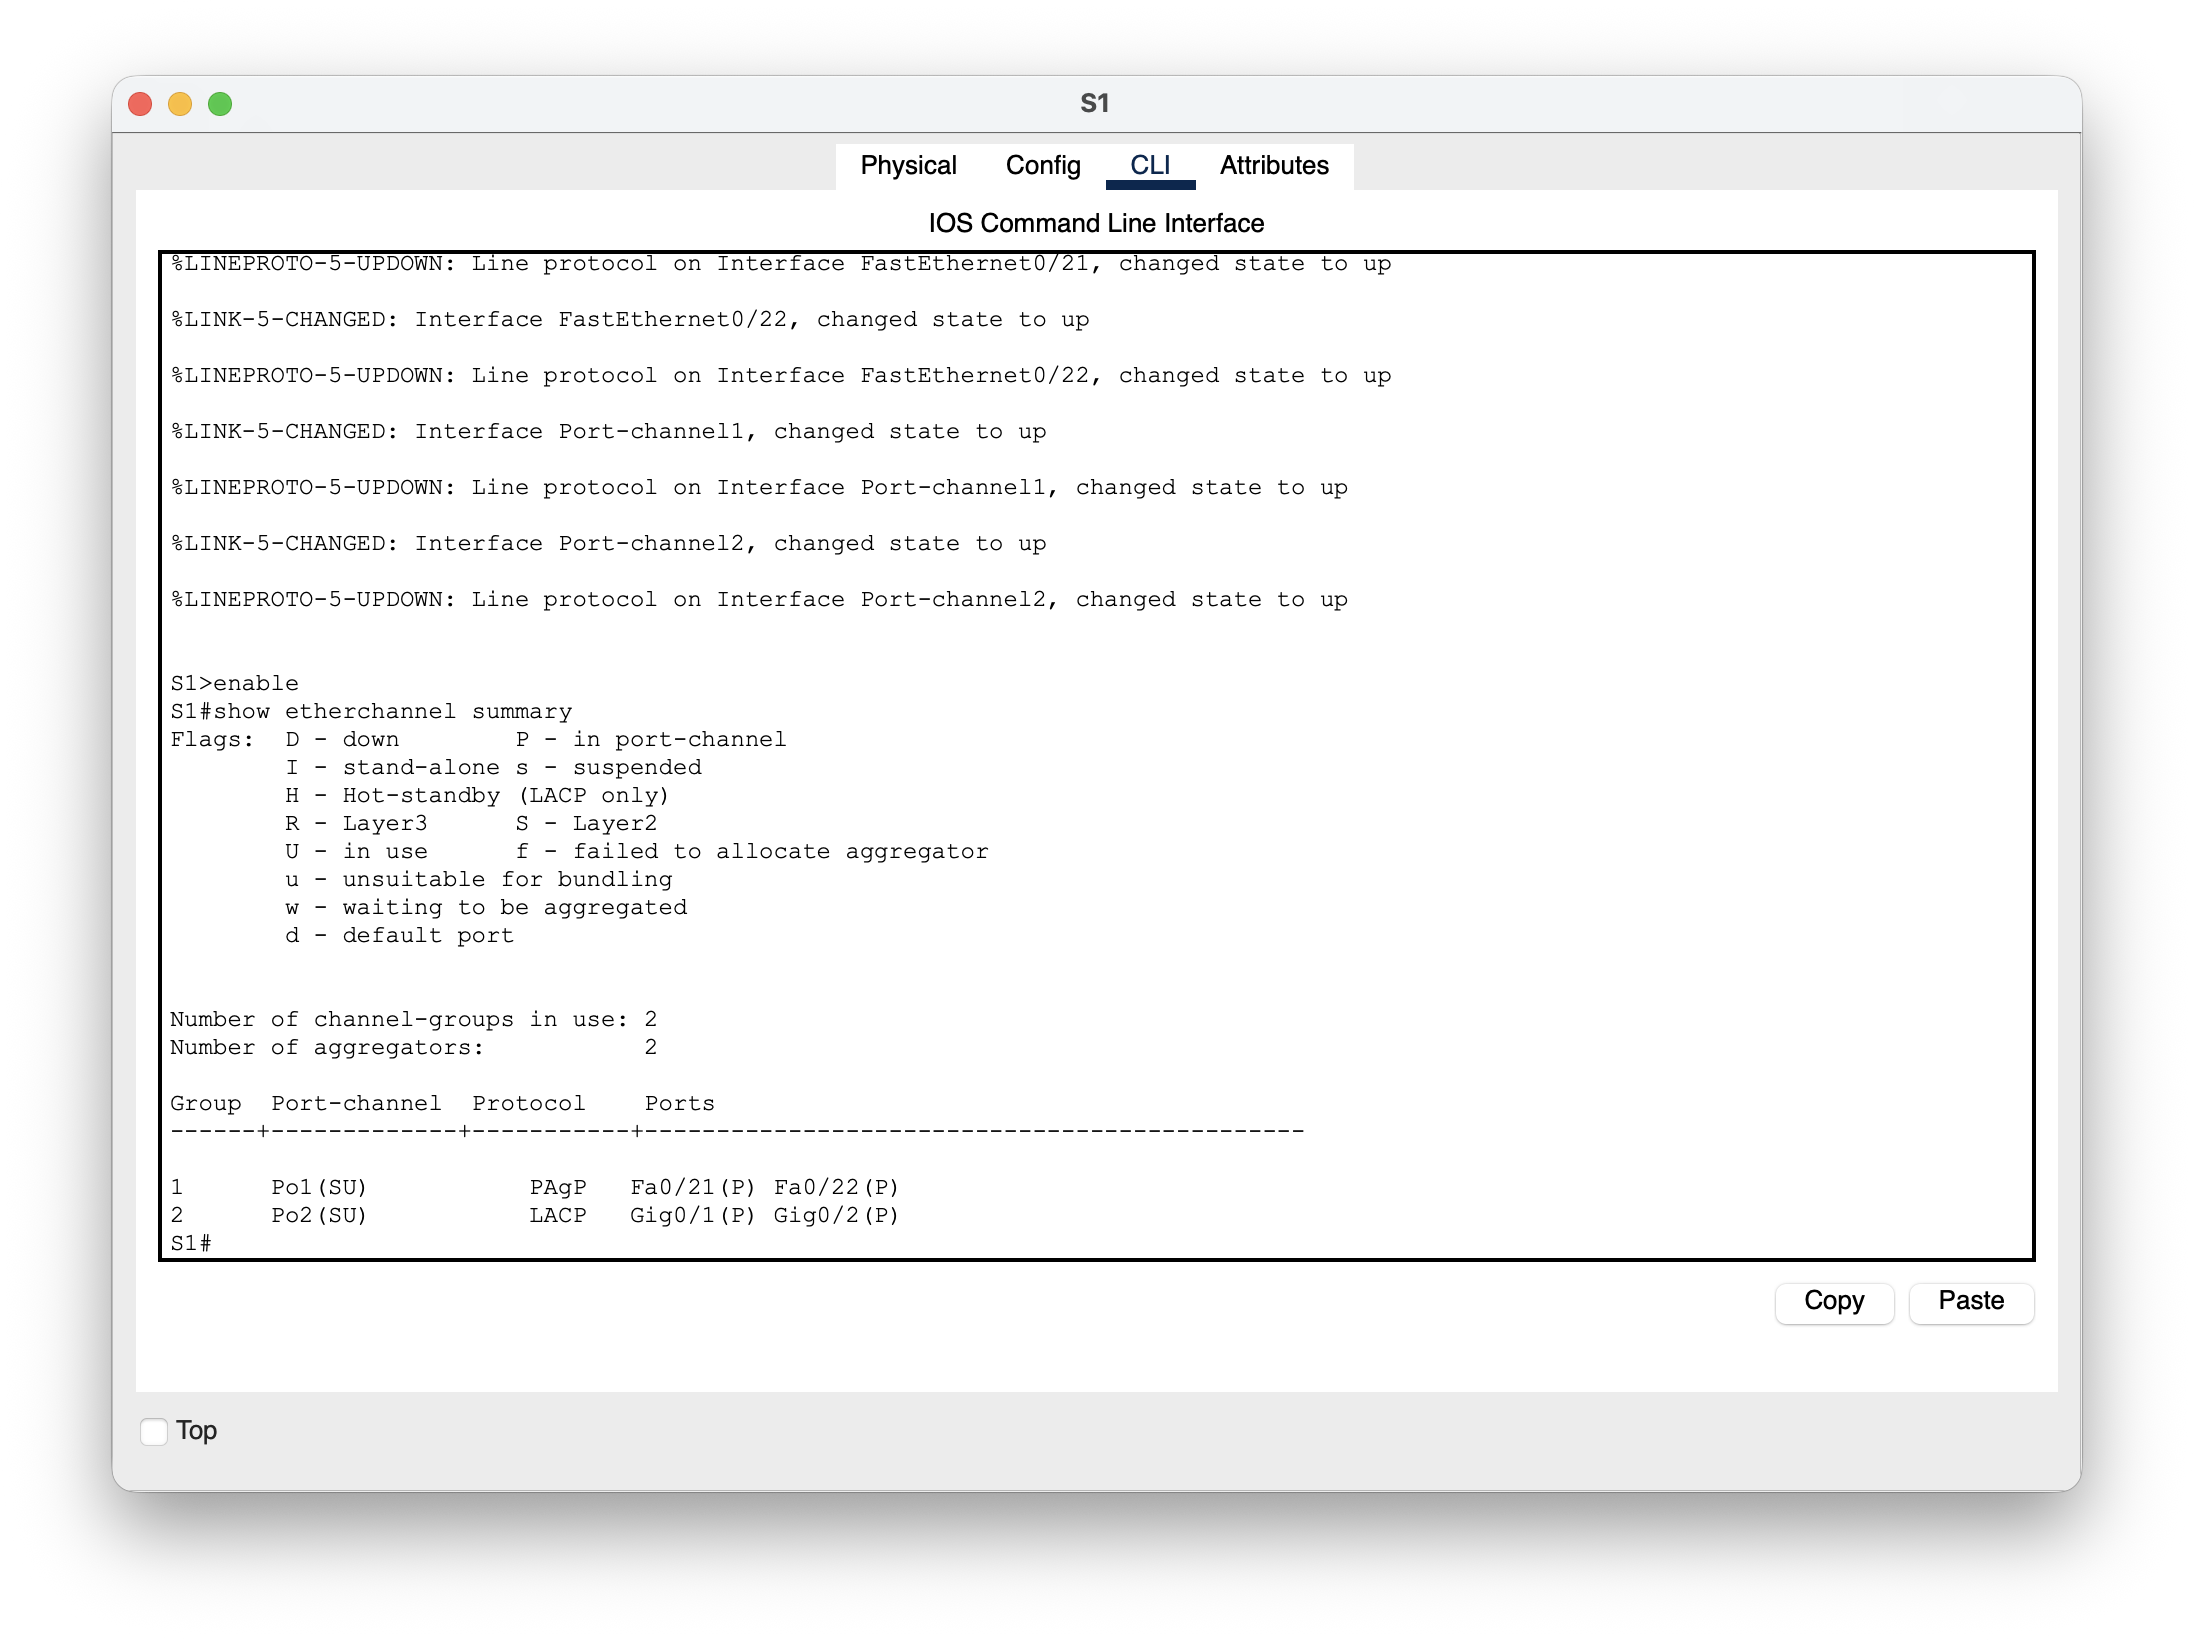
\includegraphics[width=0.8\textwidth]{confS1.png}
  \end{center}
  \caption{Configuración etherchannel en S1}\label{fig:confS1}
\end{figure}

\begin{figure}[H]
  \begin{center}
    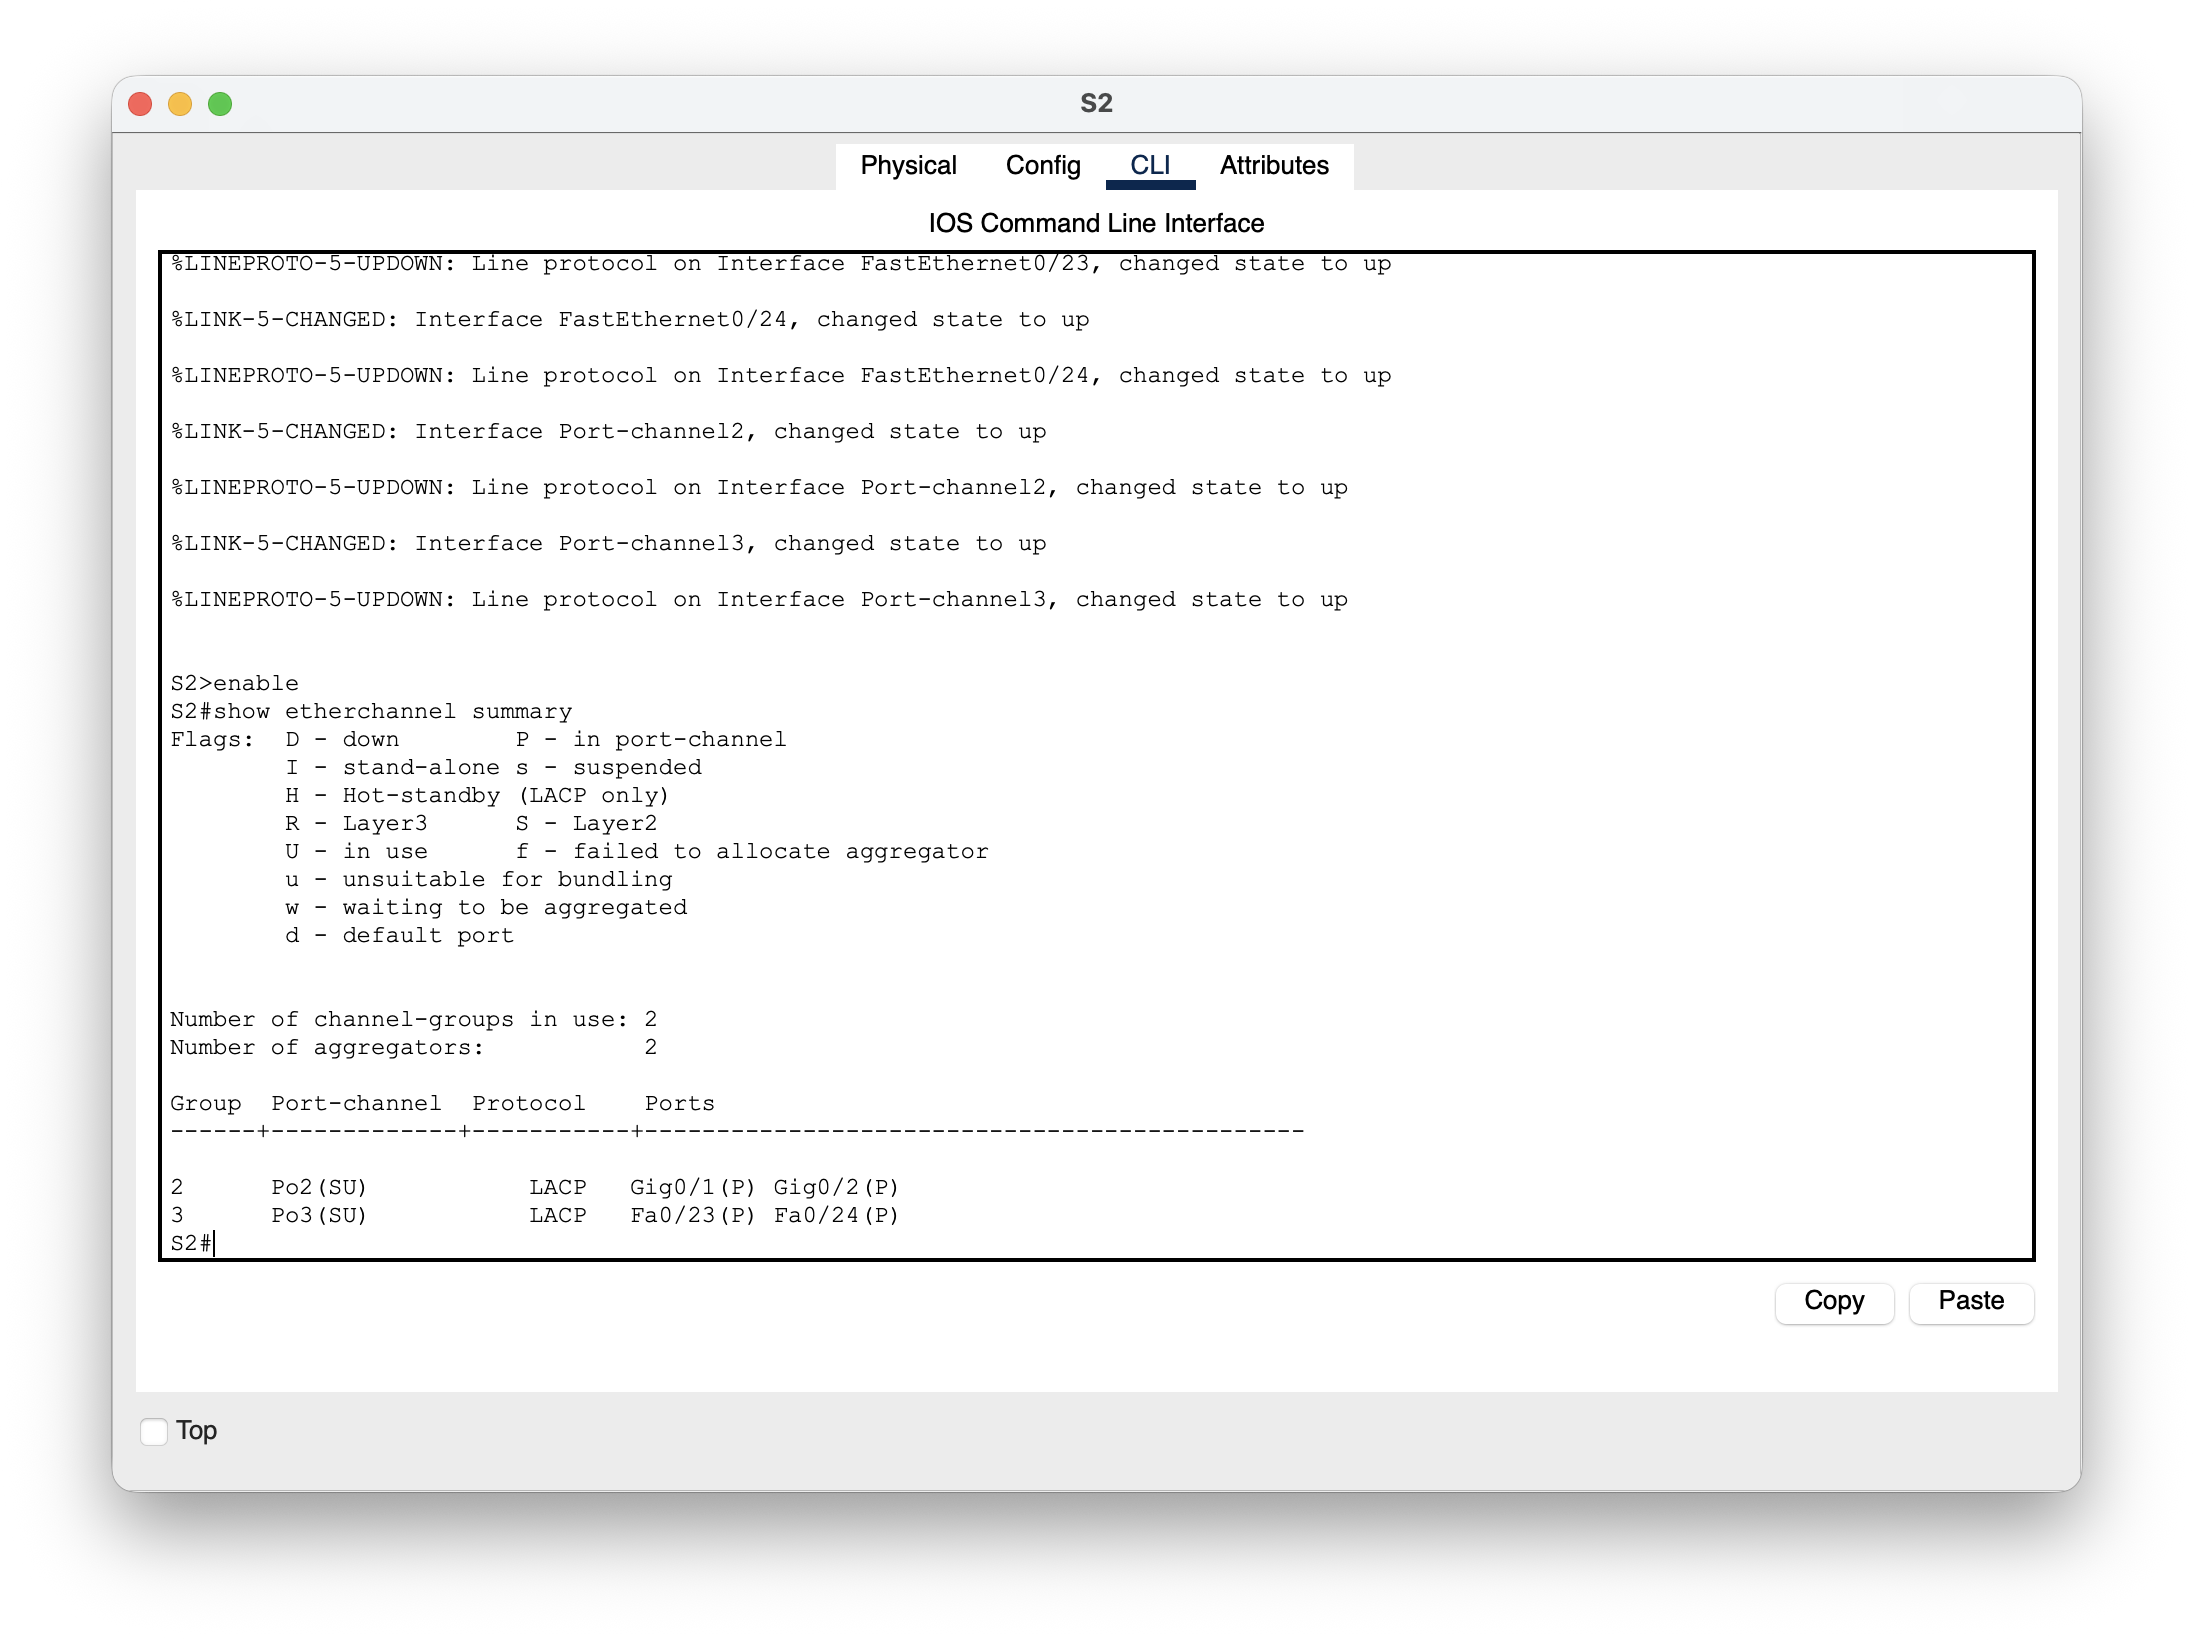
\includegraphics[width=0.8\textwidth]{confS2.png}
  \end{center}
  \caption{Configuración etherchannel en S2}\label{fig:confS2}
\end{figure}

\begin{figure}[H]
  \begin{center}
    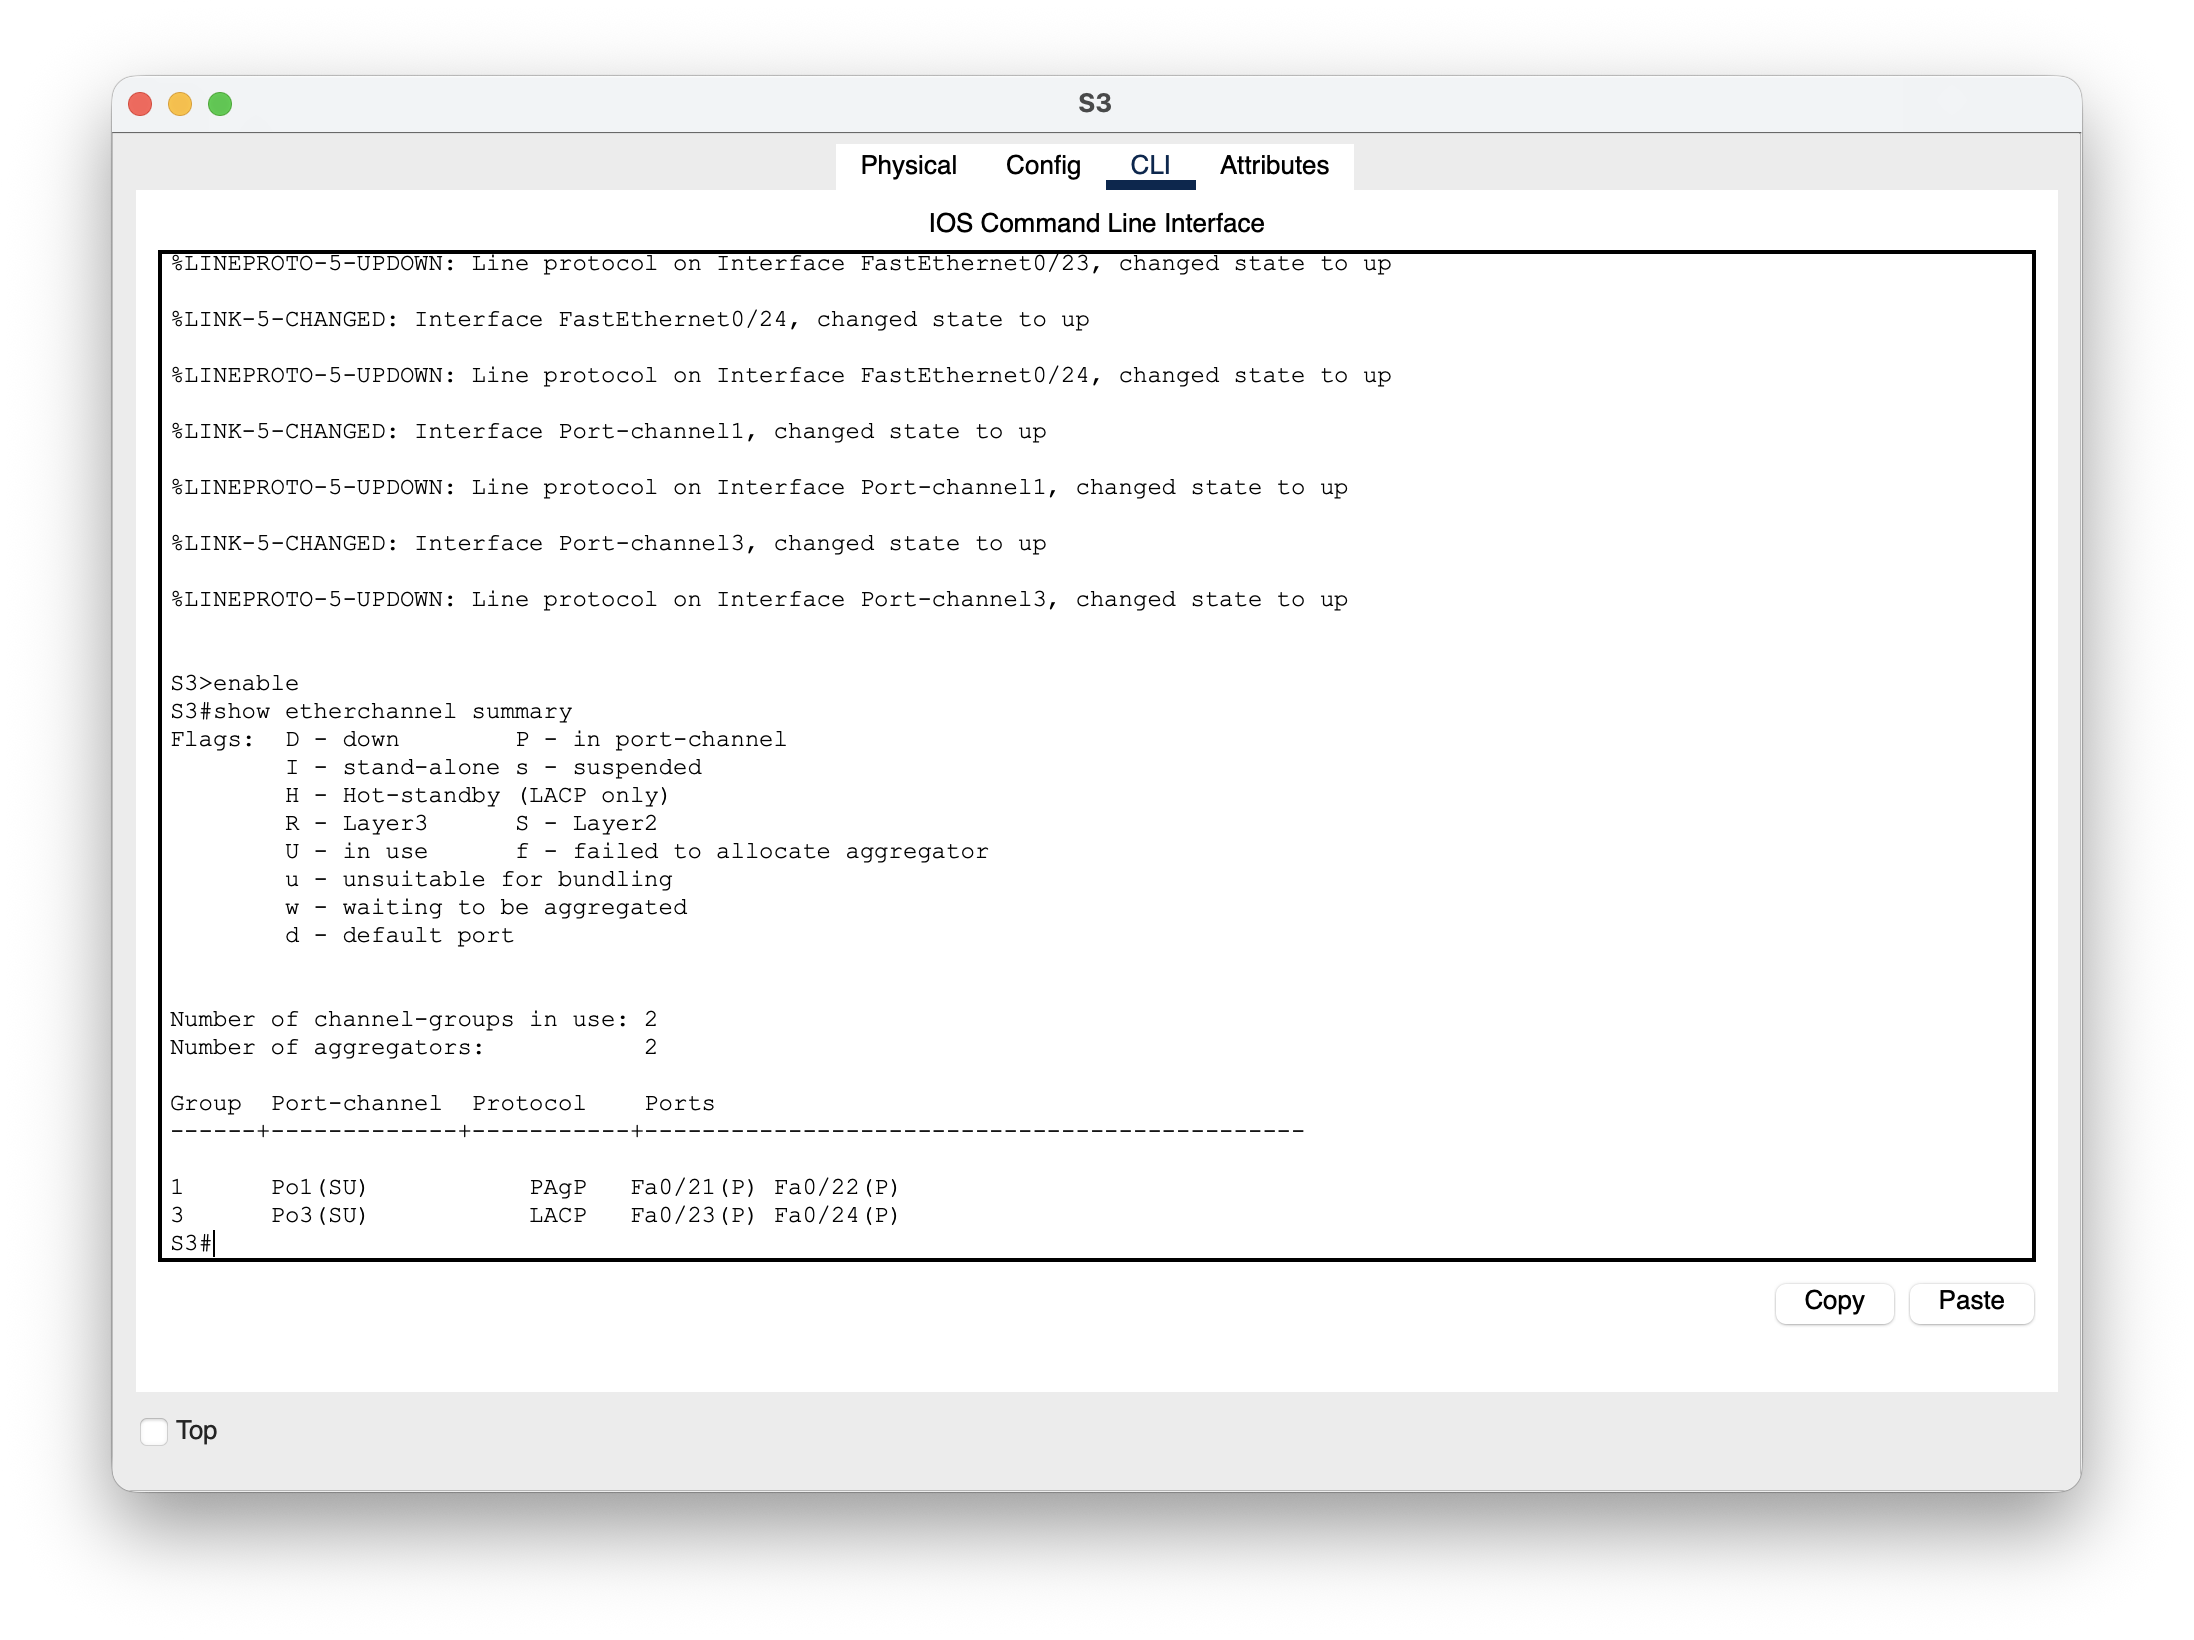
\includegraphics[width=0.8\textwidth]{confS3.png}
  \end{center}
  \caption{Configuración etherchannel en S3}\label{fig:confS3}
\end{figure}

\section{Resultados de la práctica}
En las figuras \ref{fig:results1} y \ref{fig:results2} se observan capturas de pantalla del resultado de la práctica, en la que se 
realizó todo lo solicitado, obteniendo un 100\%.

\begin{figure}[H]
  \begin{center}
    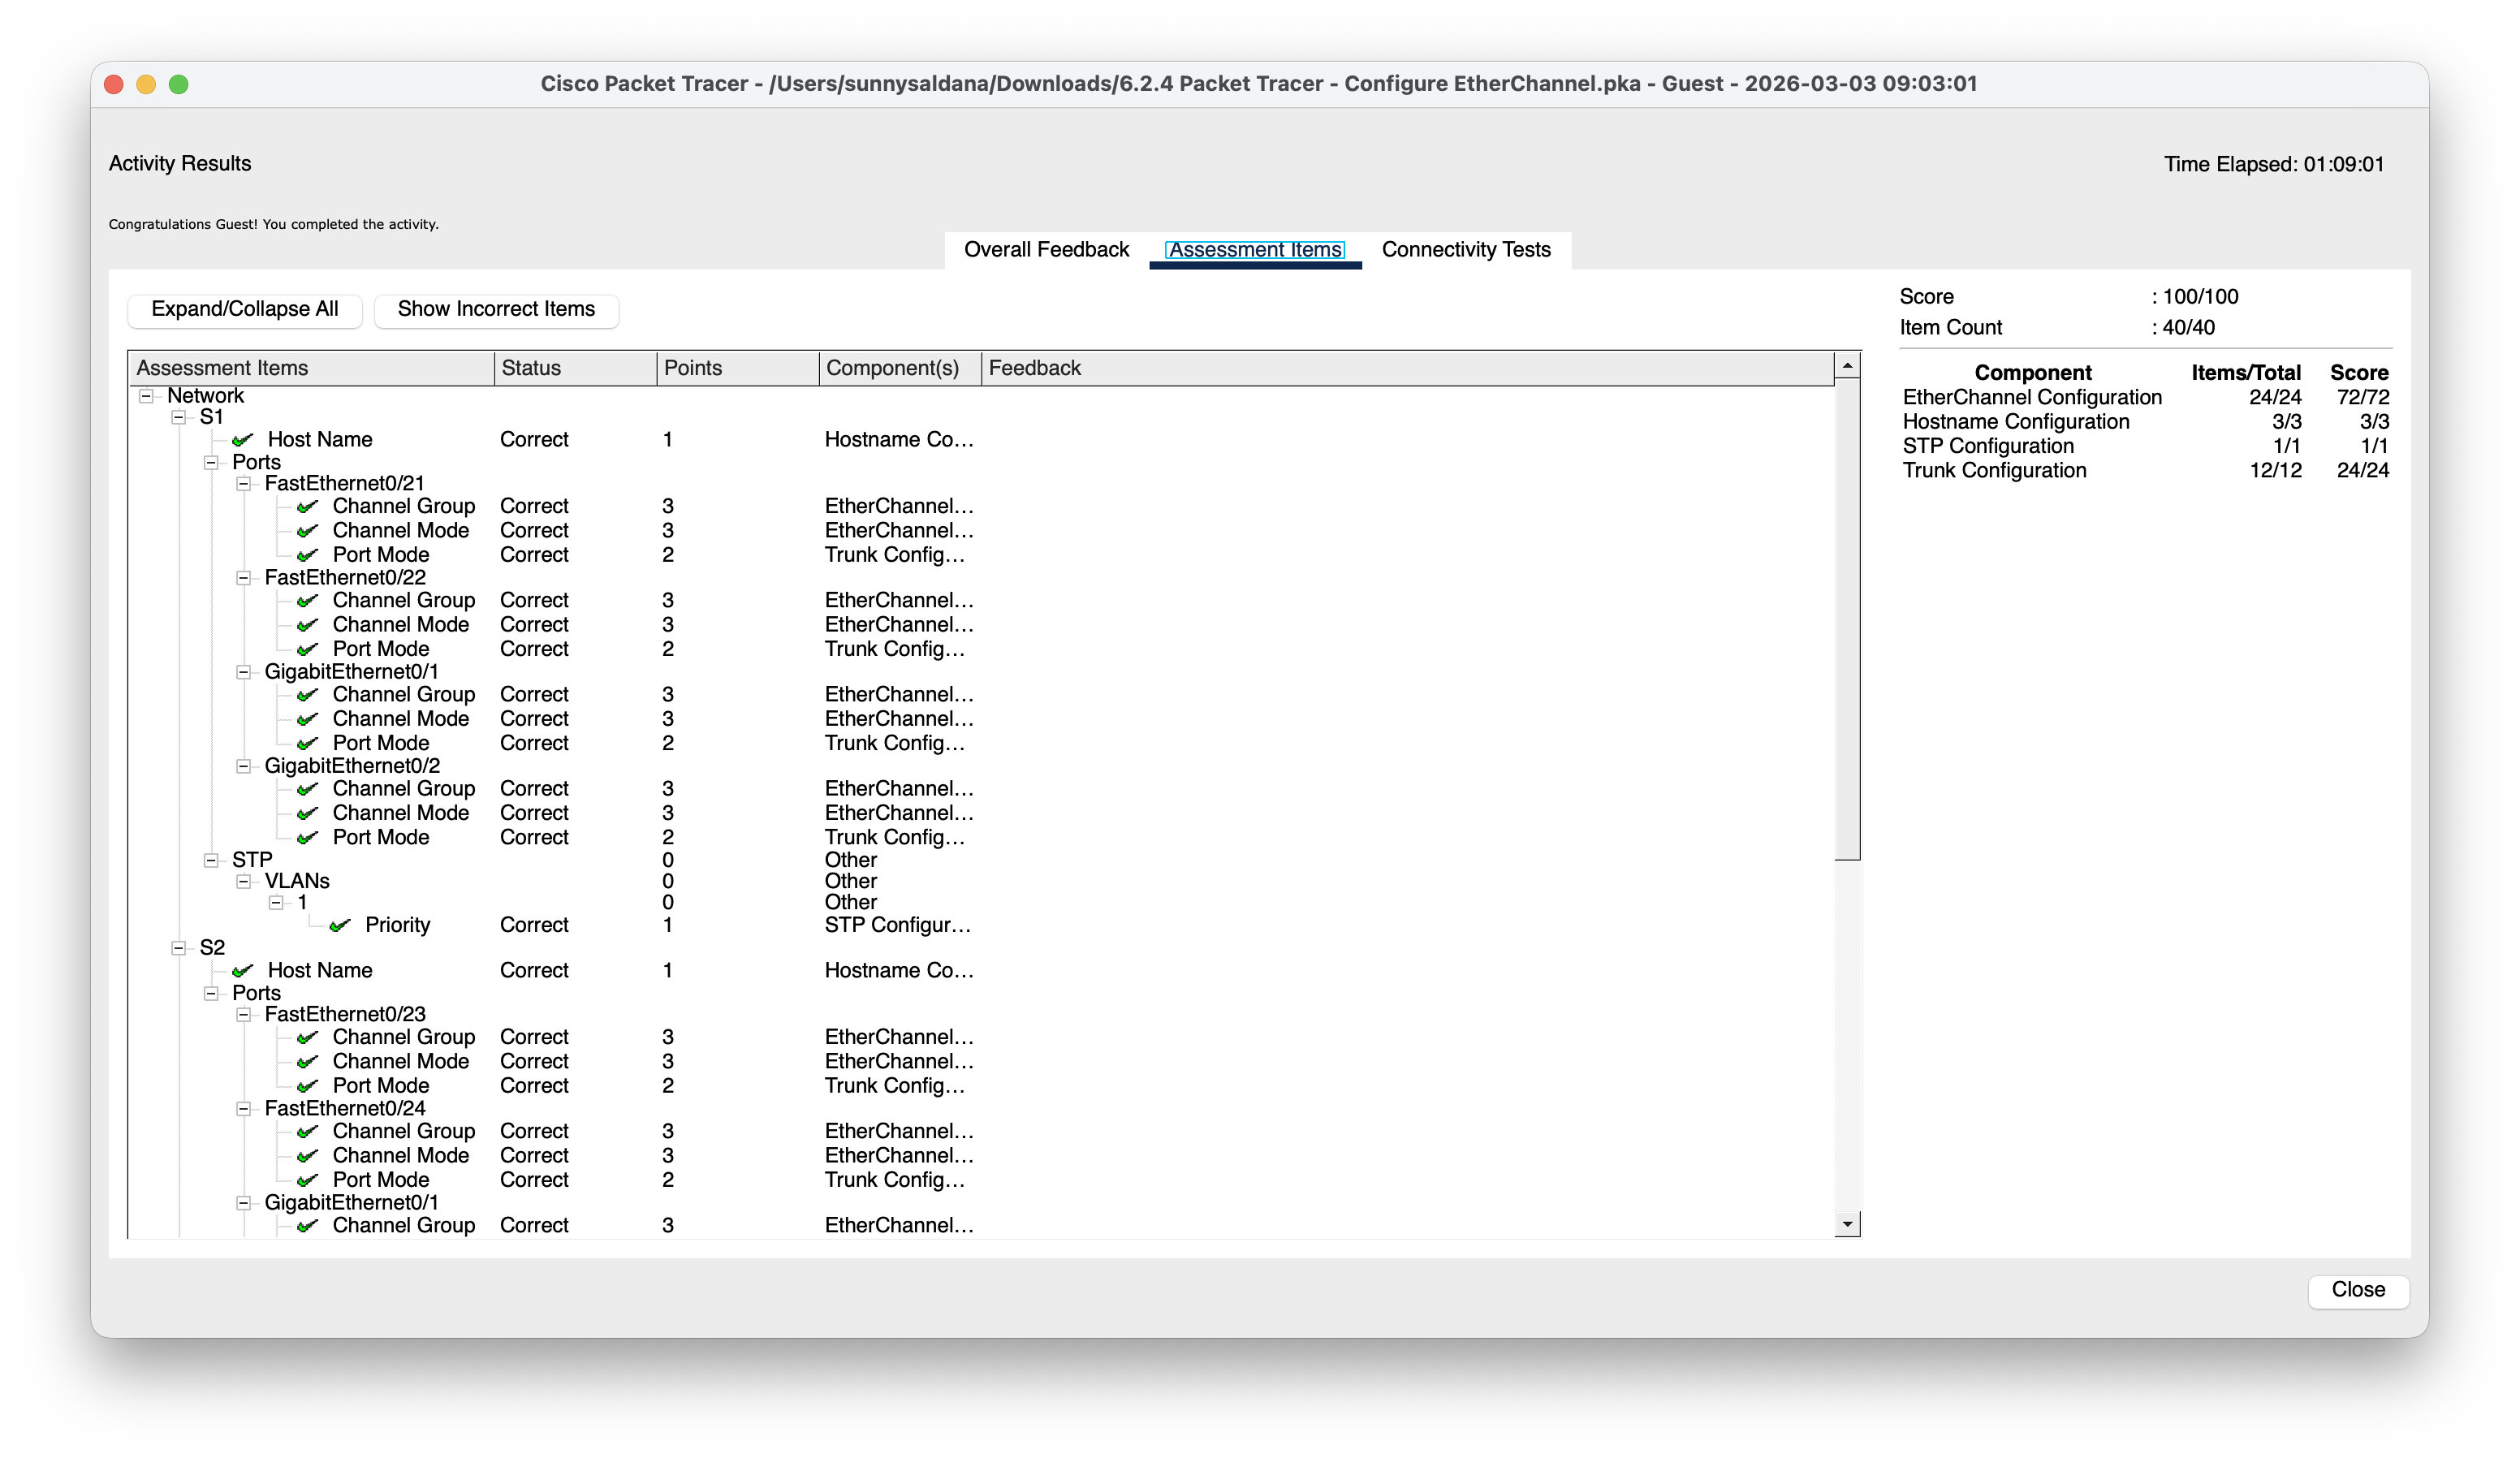
\includegraphics[width=0.8\textwidth]{results1.png}
  \end{center}
  \caption{Resultados de la práctica}\label{fig:results1}
\end{figure}

\begin{figure}[H]
  \begin{center}
    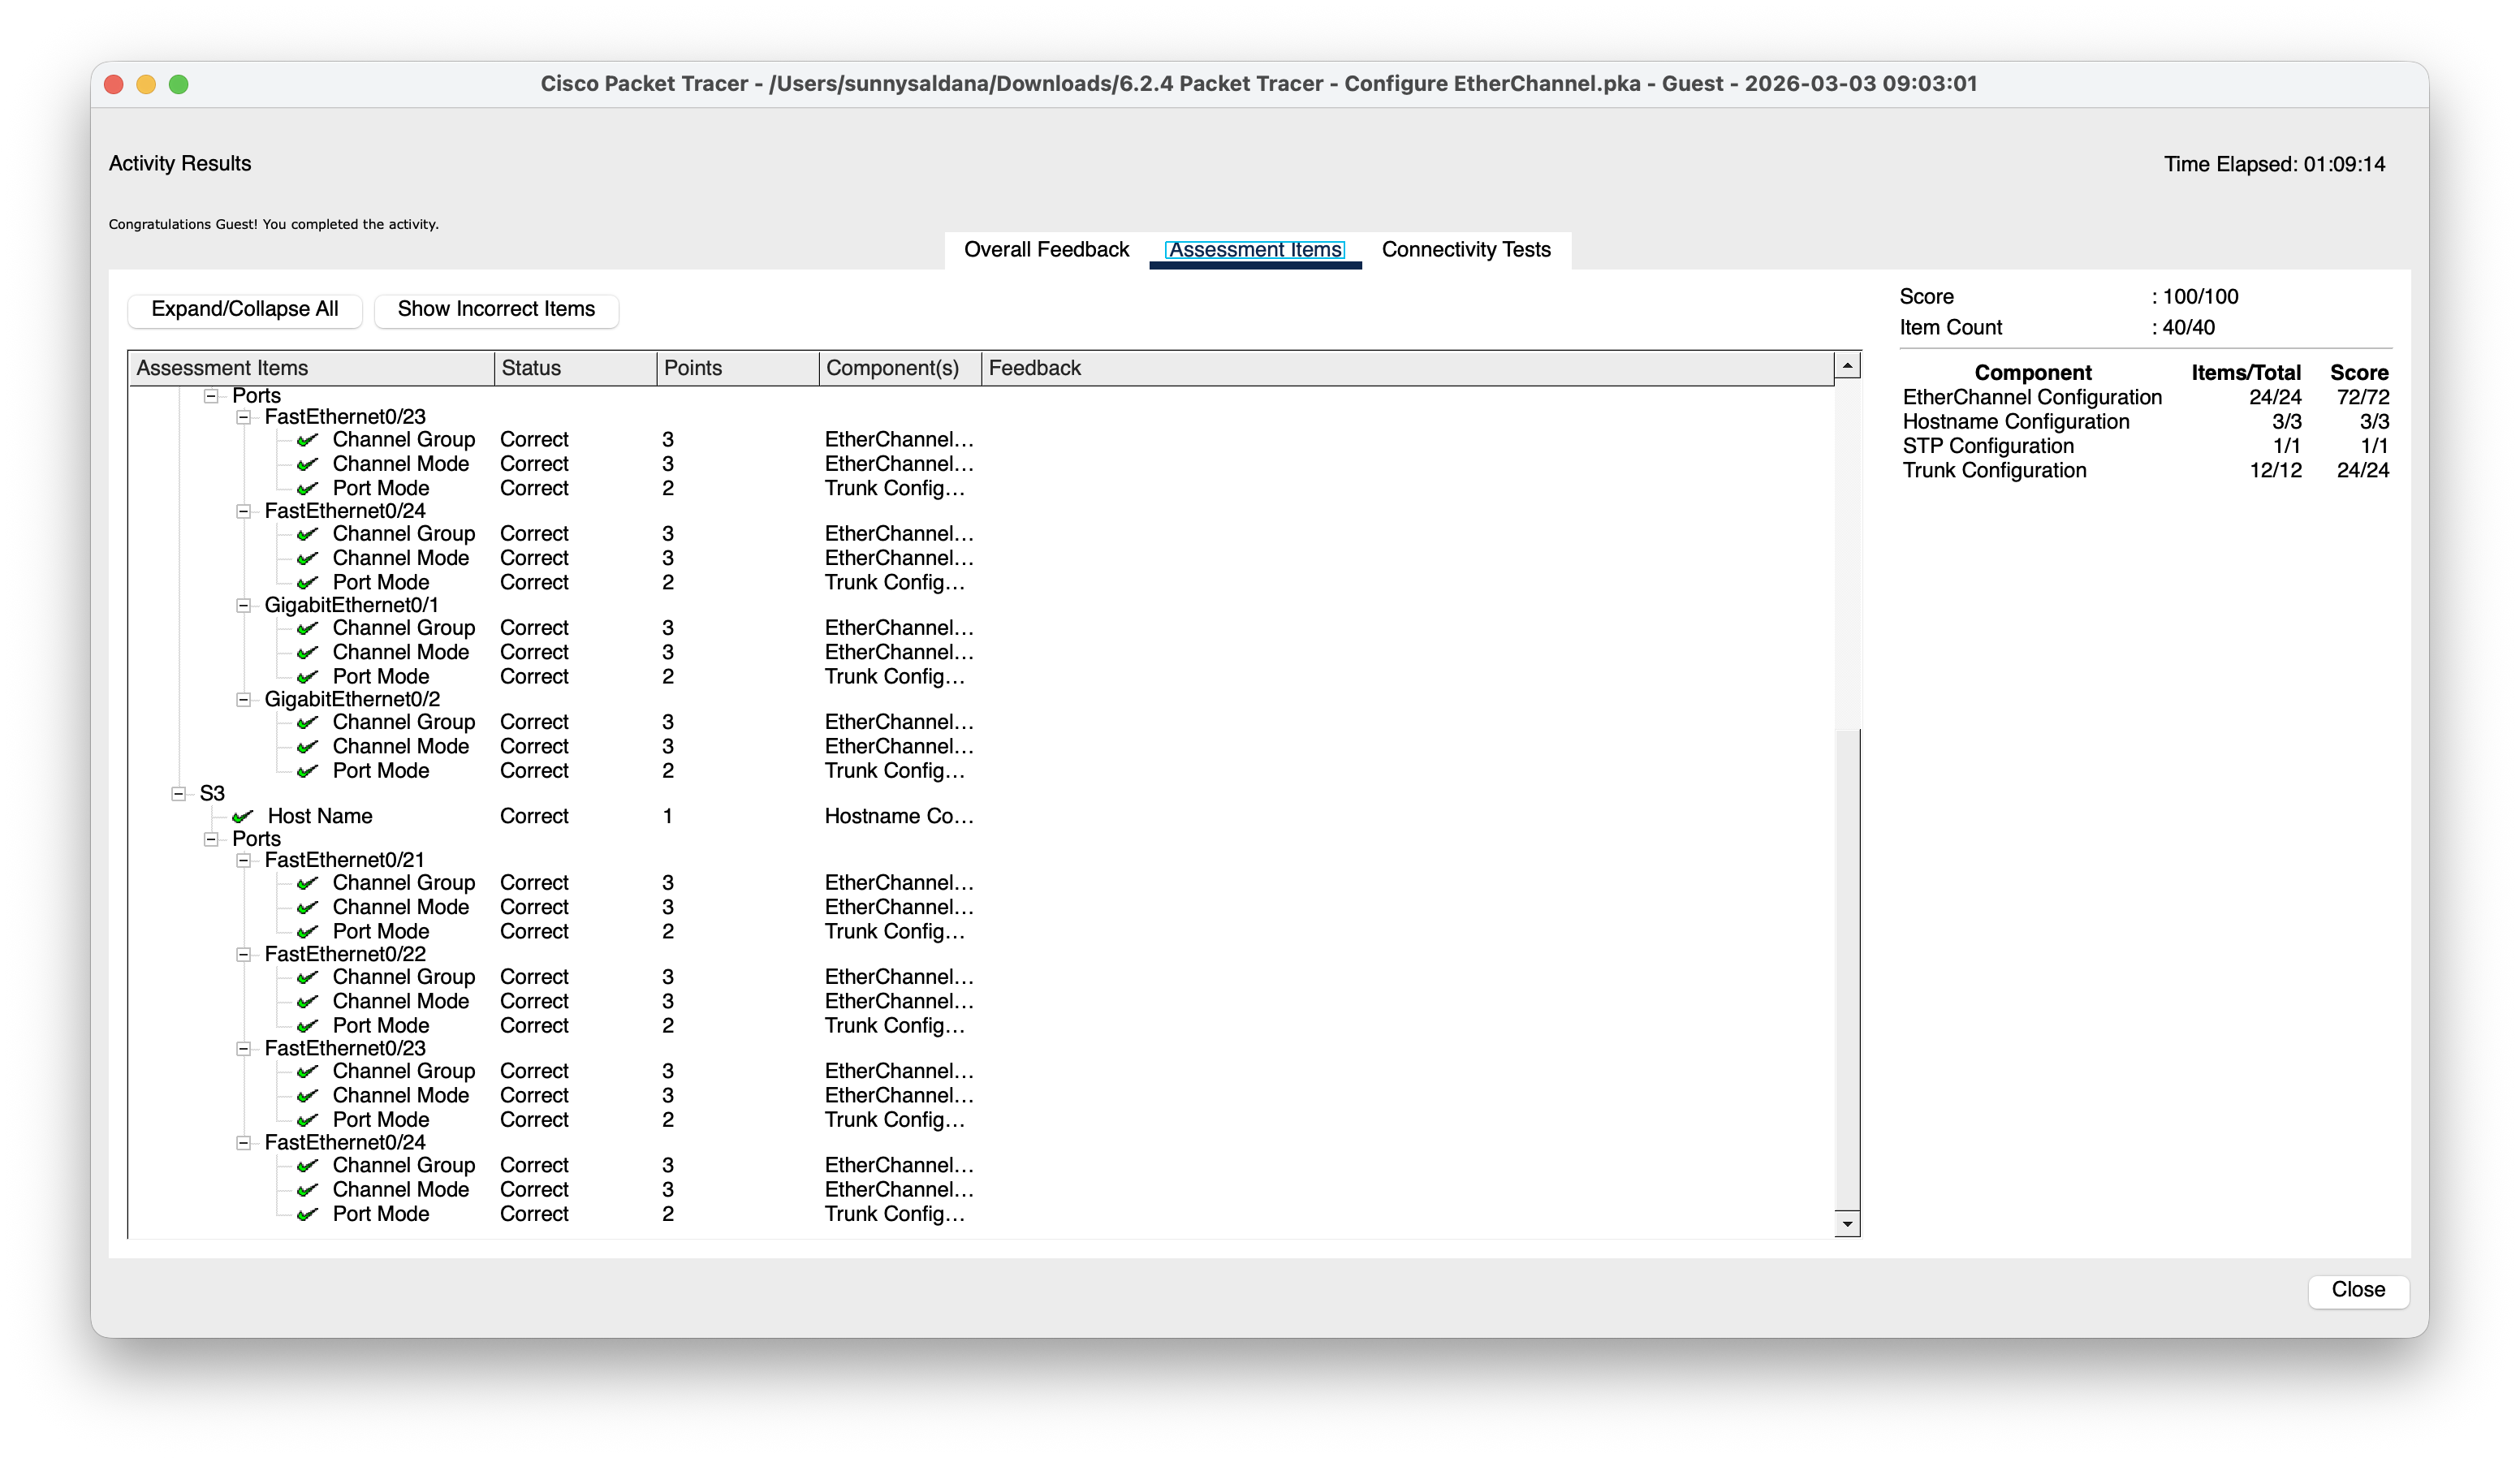
\includegraphics[width=0.8\textwidth]{results2.png}
  \end{center}
  \caption{Resultados de la práctica (continuación)}\label{fig:results2}
\end{figure}


\end{document}
